\chapter{Introduction and Background Information}
\section{Motivation}
\label{sec:Motivation}
The motivation of this thesis is to show the methodology that can be used by both applied researchers and clinicians to draw meaningful survival and causal inference from observational data with missingness. While all three fields (missing data, survival analysis, and causal analysis) are well studied, their interaction is not. I want the methods to be easy enough to describe to someone with a limited statistical background, but meaningful and valid so that the results obtained can be used in publication. The desire to have it this way stems from working on a related project with both statisticians and clinicians. While this thesis is motivated by cancer data, I believe that the methods used in this thesis are general enough to be applied to other types of data and situations.

\label{ch:Intro}
Missing data is a major problem in both statistics and medicine; however, it has not received attention proportional to its need. Survival analysis is well studied, but is relatively complete, so new research is seldom produced. Propensity score analysis will help us determine causal relationships when we don't have a randomized controlled experiment. As one could imagine, all three of these fields are important to the applied statistician, as they will come across issues in each discipline at least one at some point in their career.  The goal of this thesis is to demonstrate how to use all three in trio, a topic that has only received little interest in the literature.

In Chapter 1 of this thesis, each of these three disciplines will be described in detail separately. In Chapter 2, the methodology for using all three of them together will be discussed. In Chapter 3, the methods will be applied to a cancer dataset. Finally, in chapters 4 and 5 the implications and conclusions will be discussed.


\section{Missing Data}
\label{sec:Imputation}
In an ideal world, we would have complete data with no missingness; however this is rarely ever the case. To be specific about the definition of the word, missing data/missingness is when a subject's data for a collected covariate was not obtained. Missing data \textit{is not} when a covariate is never collected, and then suddenly the researcher wishes he had collected it. Imputation (specifically multiple imputation) is a way to ``fill in missing data'' with plausible values, and it forms the base of this thesis. Imputation itself has been around since the 1930's \cite{VanBuuren2012}, but multiple imputation is a recent development, proposed in the 1970's and formalized in 1987 by Donald Rubin \cite{Rubin1987}. To understand the use and importance of multiple imputation, we need to understand the problem of missing data, and the previous attempts to deal with it.

At first, statisticians paid no attention to missing data, and happily discarded records from their data that were incomplete. This procedure is known as Complete Case (CC) analysis. There are many problems with this paradigm. To begin with, you will lose a lot of statistical power under CC analysis, because you are throwing away records and thus decreasing your sample size. In addition, this can be costly (in terms of time or money) to the researcher, because they had to actually obtain these records that are not used. Lastly, and most importantly, any estimate obtained from a CC analysis is likely to be biased.  For example, suppose we have a random sample of people and are testing a drug's efficacy, and want to run a regression on some collected covariates. If men are known to not want to give all of their information, in the analysis, we will need to discard the male samples because they are incomplete, leaving us only with women. Thus, we no longer have a random sample, and will get biased results because we have knowingly thrown away half of our data which we know to be different \cite{VanBuuren2012}.

A slight improvement on this is called Available Case (AC) analysis. In this setting, a record is used in the analysis if it has all of the needed information for that analysis at hand. So, a record could have missingness, but if the covariate with missingness is never used in the analysis, the record will not be discarded. This paradigm is the standard analysis type for most statistical packages. It is better than CC analysis, but is still flawed. We are still throwing away valuable data as we were with complete case analysis, although likely not as much. AC analysis will still lead to bias in the same way that complete case did too. As well, new complications arise in AC analysis, namely that nonsensical situations like correlations outside of $\pm 1$, and inconsistent sample sizes between different analyses.


The next wave of statisticians in the early $20^{th}$ century wanted to improve upon available case analysis, so they developed what we now call today (single) imputation. Their goal was to fill in missing values with a single plausible replacement value. A single method (such as regression, taking the mean, resampling, etc.) is used one time to impute or fill in the missing value, and to account for the uncertainty, degrees of freedom are deducted in the following analysis. While this is a little better than complete case analysis, it still has many drawbacks. Asserting that a single value is the true value is unjustified. There is always some amount of error and uncertainty involved, and we can in no way be 100\% confident that our imputed value is correct. Furthermore, if I impute one value and you impute another, we may get completely different results from analysis on the data. This is obviously not a desirable trait.  In addition, one single imputed dataset will artificially increase your sample size. You are in effect treating the imputed values as if they were real, inflating your sample size with data that was not actually observed. This will give you unjustified statistical power and accuracy. While single imputation certainly has its drawbacks, the idea of actually trying to fill in the data (rather than throwing it away) is an important one, and multiple imputation fills in the gaps that single imputation is not able to cover.


Multiple imputation (MI) began in the 1970's, but it wasn't until 1987 when Donald Rubin formalized multiple imputation methodology in his seminal book \emph{Multiple Imputation for Nonresponse in Surveys} did it start to gain acceptance \cite{Rubin1987}. The central idea is to frame the problem in a Bayesian framework, and produce $m\geq 2$ values to substitute in for each missing value, drawing these values from the missing covariates posterior distribution. Using these $m$ substitute values, we can think of the data now as being $m$ datasets, each dataset containing the observed data, and one value for each piece of missing data. 


An example will make the MI process clear. Suppose that we had a dataset of age, weight, and height. We want to do a linear regression of weight on age but we have missingness in weight and height. First, we will impute our data (figure \ref{fig:miexample}, the first two columns). Once we have a sufficient number of datasets (we will talk about how to pick the number later), we can run the regression analysis on each of the MI datasets, treating the dataset as if it was complete (horizontal lines and third column). After running the model on the $m$ datasets, we can pool the results to get one single estimate with its associated variance (last column).  We will speak of the exact details of the MI process in detail in the second chapter.
\begin{figure}[!ht]
  \centering
    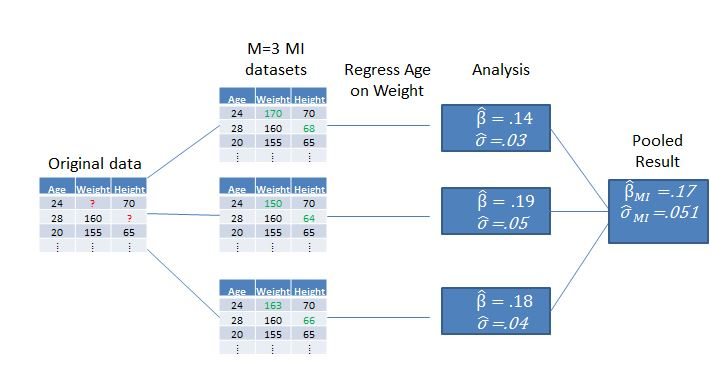
\includegraphics[width=0.85\textwidth]{mi_example_full.jpg}
  \caption{Example of the MI process}
\label{fig:miexample}
\medskip
\small
In the original data, missingness is displayed by \textcolor{red}{?'s} and the imputed data is shown in the multiply imputed data as \textcolor{green}{\#'s}. We then regress weight on age in each MI dataset, get the results from each, and then pool them together.
\end{figure}


The MI method is obviously much better than the previous attempts to correct for missing data because it permits us to keep the data we already have, as well as to quantify our uncertainty about imputing the missing values.  

The use of MI has been steadily increasing over the past 30 years, and it is now the standard for missing data. It has seen a great increase in use in the medical field, but has yet to see mainstream success in the statistical community. 
\begin{comment}
Stef van Burren, an influential author in multiple imputation did a study of academic papers, and concluded that the number of publications using or mentioning multiple imputation is growing at an exponential rate since about 1990 \cite{VanBuuren2012}. Thus, using multiple imputation to handle missing data will be advised because of its popularity and strength.
\end{comment}



\section{Survival Analysis}
\label{sec:Survival}
Survival analysis is a large and important field in statistics, and there have been many textbooks written about it. I only plan to introduce the topics that are relevant to my case study; for a much more detailed account of survival analysis, please see reference \cite{Klein1984}.


Survival analysis on the whole can generally be described as the analysis of time to event data, often in the presence of censoring (when we don't have complete information about the time of event).  There are many techniques used in this field, but the main tools that we will be using are Kaplan-Meier estimates, log rank tests, and Cox regression. 


Before we go on, it should be noted that often in the literature and software (and in this paper) we see terms like ``death/failure'' and ``survivors''. This is due to survival analysis being heavily influenced and intertwined with medical studies. A more general term for these would be ``event'' and ``those who have not had an event yet''. These terms are used because they are clear and concise, although it might not accurately describe the event at hand. For example, if we were tracking the time until a child loses all of their baby teeth, the term death would obviously not portray the event of interest, but may be used in the context to denote losing all of the teeth.

The Kaplan-Meier (KM) estimator is a nonparametric estimate of the true survival function (the probability of survival after time $t$, $S(t)=P(T>t)=\int_t^\infty f(u)du$, where $f(u)$ is the unknown probability density function). It is defined as 
$$\hat{S}(t)=\prod_{t_i<t}\frac{n_i-d_i}{n_i}$$
where $n_i$ is the risk set, defined as the number of people who have not had the event or been censored right before time $t_i$ ,and $d_i$ is the number of deaths observed at time $t_i$ \cite{Kaplan1958}. The Kaplan-Meier estimator is very commonly used as a measure to see how different treatments affect the survival of the population in question, and is helpful in seeing at what time points survival changes the most (i.e. early or late). 

Knowing the shape of the Kaplan-Meier curve is interesting and gives a good graphical representation of survival over time, but it would be wise to have a statistical test to compare survival two curves. The log rank test is a popular nonparametric test that researchers often use to see if two or more survival curves come from the same distribution \cite{Bland2004}. This is a useful tool to have, because visualizing curves alone does not give us this information. We could have two curves that look radically different due to sampling error, yet still come from the same distribution.
\begin{comment}
 Knowing whether the survival curves come from the same or different distribution is useful because it allows us to make statements like ``drug A is associated with longer survival time than drug B''.
\end{comment}


The general log rank test is defined as:
$$\frac{\sum_{j=1}^{J}w_j(O_{1j}-E_{1j})}{\sqrt{\sum_{j=1}^{j}w_j^2V_{j}}}\sim N(0,1)$$
Where $w_j$ is the weight of each individual (must be $\geq 0$, we will set all to be 1), and $N_j=N_{1j}+N_{2j}$ is the number of subjects in the risk set at time j, composed from the sum of the number of deaths at time j in each group, $O_j=O_{1j}+O_{2j}$ is the observed number of deaths at time j, composed of the sum of deaths from either group at time j,  which leads to the desired quantities $E_{1j}=\frac{O_jN_{1j}}{N_j}$ , and $V_j=\frac{O_j(N_{1j}/N_j)(1-N_{1j}/N_j)(N_j � 0_j)}{N_j -1}$.


Typically, all of the weights are set to one, as this test places equal weight to all of the deaths we observe. We could change these weights though to give more emphasis to certain death times. This is useful for example if we have a drug that takes a long time to start working. We wouldn't care about early deaths, only about later times when we are comparing the survival. Putting more weight on the later deaths would help to answer this question better. It can be proven that the log rank test is equivalent to the score test on a Cox model (which will be discussed next) fit the same data with no tied event times, and very similar when there are ties \cite{Klein1984}.

Proportional hazards regression, often called Cox regression or Cox model is a modelling tool that allows us to analyze the hazard ratio of a covariate, assuming that each covariate acts to multiply the hazard ratio. 


In order to understand Cox regression, we first need to learn about the hazard function. The hazard function is a survival tool that tells us the \textit{rate} of events at time $t$, conditional on survivorship until time $t$. Mathematically, it is given by:
$$\lambda(t)=\lim_{\Delta t\rightarrow 0+}\frac{P[t\leq T<t+\Delta t|t \leq T]}{\Delta t}.$$
Cox regression is a maximum (partial) likelihood method estimator, given by: 
$$h(t|Z)=h_{0}(t)\exp(\sum_{k=1}^{p}\beta_{k}Z_{k}).$$
where $h_0(t)$ is what's known as the baseline hazard, and can be any positive function. Note how it only depends on time and not any covariates.  Z is a vector of observed covariates, and does not depend on time. The $\beta$'s are found by maximizing the partial likelihood function
$$L(\beta)=\prod_{i=1}^{D}\frac{\exp(\sum_{k=1}^{p}\beta_{k}Z_{(i)k})}{\sum_{j\in R(t_{i})}\exp(\sum_{k=1}^{p}\beta_{k}Z_{jk})}$$
Where $Z_{(i)k}$ is subject $i$'s kth covariate, $R(t_j)$ is the risk set (set of those who have not died yet at the time just prior to $t_j$), D is the number of distinct death times and $p$ is the total number of covariates in the model \cite{Cox1972}.


Our inference of interest is on the hazard ratio, given by 
$\frac{h(t|Z)}{h(t|Z^{*})}=\exp(\sum_{k=1}^{p}\beta_{k}(Z_{k}-Z_{k}^{*}))$,
where Z* is another set of covariates. The hazard ratio describes how the hazard changes between individuals with different covariates. Often times, the interest lies in what happens when all covariates are held constant, and the covariate of interest is increased one unit (or if a categorical variable, changing groups). This ratio will be a constant, and should not vary over time; hence the name proportional hazards. This is so because the ratio does not depend on the baseline hazard (which cancels out when taking the ratio). Using Cox regression, statements such as   ``Increasing the drug by one \textit{mg} will decrease the rate of death (compared to non-users) by 30\%''. Cox modelling is one of the most used models in the survival and medical literature, because it is flexible, powerful, easy to use, and incorporates other covariates into the survival model.

\section{Causal Analysis}
\label{sec:PSA}

In an ideal world we would like to be able to do research and say that A causes B, rather than ``our study says that A is associated with B''.  However, the only way to get this interpretation is if we conduct a Randomized Controlled Trial (RCT). Although we can analyze any observational data using survival analysis, unless an RCT is conducted, we can only make claims about association, not causation. In order to prove causality, we need experimental data in a randomized and controlled setting, not observational data. The reason for this is because in an RCT, we expect the groups to be similar at baseline (due to randomization), and thus any differences between the groups after treatment should only be related to the treatment. However, in an observational study (where treatment assignment is not random, and may even by chosen by the participant), we have no reason to believe the groups are similar at baseline (in fact, they might be systematically different), and the difference after treatment could be due to the treatment or something else. 


Randomized controlled trial is a term that is often thrown around, but I want to be precise with its definition. An RCT is a study design that ``randomly assigns participants into an experimental group or a control group. As the study is conducted, the only expected difference between the control and experimental groups in an RCT is the outcome variable being studied'' \cite{RCT2011}. This is in stark contrast to a retrospective study of observational data, where historic data of people who chose what group/treatment they wanted to be in are studied. When making judgment on a retrospective study, we cannot be sure if the differences between the groups are due to their treatment choice, or some other factor. RCT's are the gold standard for experiments, and should be used if possible when trying to study causality. But often times monetary, ethical, and other factors prevent us from doing so. In this case, the best data we may be able to get is retrospective observational study. 


Luckily, we can still analyze observational data for causality. We can frame our problem in a framework known as the Rubin Causal Model, which helps get causal understanding from non-experimental settings \cite{Guo2010}. Rubin's causal model is built upon the idea of a counterfactual, also known as a potential outcome. Put simply, the counterfactual is the result that we would have observed had the subject been in the other group. For example, if we were testing a weight loss drug versus a diet in a study to see which lead to more weight loss, if subject 1 took the drug, then his observed value would be the weight lost on the drug, whereas his counterfactual would be the weight lost had he dieted. Together, the observed value and the counterfactual form what is known as the potential outcomes. For the $i^{th}$ subject, the potential outcomes are denoted as $Y_i(0),Y_i(1)$, where the 0 means treatment and 1 means control. Often times, authors give the observed value concisely as $Y_i=Y_i(1)T_i+Y_0(1-T_i)$, where $T_i$ is the treatment indicator (1 means treatment, 0 means control).  In an ideal world, we would observe both potential outcomes, however, this is obviously not possible, since we can only observe one outcome. This issue is what is known as \textit{the fundamental problem of causal inference}.


Rubin's Causal Model framework relies on two assumptions. The first is called the stable unit treatment value assumption (SUTVA), which states that the potential outcome for the $i^{th}$ subject will be the same no matter what treatment the other subjects receive. The second is called ignorable treatment assignment (sometimes called no unmeasured confounders), which states that the potential outcome should be independent of the treatment assignment given the confounding factors. Put formally, this condition is $(Y_0, Y_1)\perp T|X$, where X are the pretreatment covariates confounding the potential outcomes and the treatment assignment \cite{Guo2010}. This assumption is untestable, but can be reasonably assumed in most cases if we do the propensity score analysis correctly (which we will talk about soon). This assumption is satisfied automatically in an RCT, because knowing treatment assignment doesn't give any information about the potential outcomes. If we are able to meet these assumptions, then using Rubin's causal model will help us make causal inference from non-RCT data, as we will discuss.


If we are able to get the counterfactual, we could compute the treatment effect of the treatment for each individual. However, this is not of much interest to us. Rather, we are interested in the treatment effect on the entire population, not the individual. There are two common estimands used to measure the causal effect in the population. The first is the Average Treatment Effect (ATE), and it is defined as how the treatment effect changes when the population moves between treatment groups. It is given mathematically by $E[Y(1)-Y(0)]$. The other measure is called the Average Treatment Effect on the Treated (ATT), which is the treatment effect of one group moving to another treatment is given by $E[Y(1|T=1)- Y(0|T=1)]$. 

It should be noted that unless we have the no unmeasured confounders assumption $E[Y(1)|T=1]\neq E[Y(1)]$, because $E[Y|T=1]=E[Y_1T+Y_0(1-T)|T=1]=E[Y_1|T=1]\neq E[Y(1)]$. And the same holds for $Y(0)$, such that $E[Y(0)|T=0]\neq E[Y(0)]$. If we were to use $E[Y(1)|T=1], E[Y(0)|T=0]$ as substitutes for $E[Y(1)], E[Y(0)]$ in our calculations, we would get biased estimation of the treatment effect. What this means is that if we are not in the causal framework or in an RCT, then we cannot split the expectation up and just take the mean from each group to get the causal effect. However, if we are in the causal framework, and we assume no unmeasured confounders, then $ E[Y(1)|T=1,X]= E[Y(1)]$ because the potential outcome is independent of the treatment assignment, and the same holds for the control group.  If the potential outcomes were independent of the treatment assignment (like in an RCT), then we could break apart the expectations and calculate the estimands as the difference in the expected values between the treated and control group. But since we don't get this automatically satisfied in an observational study, we need to develop methods to help us get this interpretation.
\begin{comment}
however, we note that with an observational study, $E[Y|Z=1]=E[Y_1Z+Y_0(1-Z)|Z=1]=E[Y_1|Z=1]\neq E[Y(1)]$, and the same holds for when $Z=0$ . Put formally, in an RCT, $(Y_0, Y_1)\perp Z$ holds, but not in an observational study. If we can control for all confounding pretreatment factors though (denoted by X), then we may say that $(Y_0, Y_1)\perp Z|X$. This statement is the mathematical definition of the ignorable treatment assumption of Rubin's Causal model. This is unverifiable, but if we believe that we have all of the confounding factors, then this assumption will be reasonable.
\end{comment}


The goal of randomization in RCT's is to make the groups be as similar as possible at baseline, that is, the distribution of the pretreatment covariates should not be too different. However, in an observational study, the groups may be very different. It is quite likely that some baseline factor might influence how somebody picked their treatment. In the weight loss pill example, healthier people may choose the diet over the pill, whereas people motivated to lose weight might be inclined to take the pill, so the participants in the two groups will not be similar to start with. We should try to make them more similar (i.e. balanced) if we wish to emulate an RCT. 


In order to implement balancing in Rubin's causal model, \textit{propensity score analysis} is used. The propensity score is the probability that the subject received the treatment given the pretreatment covariates that are believed to be confounded with treatment choice. The propensity score for the $i^{th}$ subject is given by $\hat{e}_i(X)=P(T_i=1|X_i=x)$ and can be found by any method that gives group membership probabilities \cite{Rosenbaum1983}. We assume that some of the pretreatment covariates confound treatment status and outcome, so controlling for this makes all of the patients seem similar at baseline. Because of the propensity score theorem, if we have ignorability, then we say that $(Y_0, Y_1)\perp Z|\hat{e}(X)$, \cite{Angrist2008}. With the no unmeasured confounders assumption, we must condition on a vector to get independence, however, the appeal of the propensity score is that we can get the same assumption by only conditioning on a scalar quantity (the propensity score).


Propensity scores lead to group balancing, that is, if propensity scores are controlled, then our groups will have a similar distribution for each baseline covariate at the start of the study. Put formally, propensity scores aim to remove the confounding between pretreatment characteristics and treatment. And thus, by controlling for propensity score and using Rubin's causal framework, we can treat the data like it was an RCT. The most popular propensity score methods are propensity score matching (where we match those who picked the treatment to those who did not based on propensity score similarity) and propensity score weighting (where each individual's contribution to the average treatment effect is dependent on the inverse of their propensity score). Propensity score matching has fallen out of favor recently because there will be some data thrown away, and the balancing that follows might not be that accurate \cite{King2015}. However, propensity score weighting is still a popular method today \cite{Lunceford2004}.


Getting the propensity score was historically done by logistic regression, although recently newer machine learning methods have been employed. Any method that will lead to probability of treatment or control membership will suffice. There has been a lot of debate as to which covariates to include in the propensity score; either all variables, or only relevant variables, but I don't aim to settle this debate in this paper. 

This paper is interested in weighting, specifically, inverse probability of treatment weight (IPTW). With IPTW, the sample is reweighted so that at baseline, the groups appear similar. These weights are given by
$$w_i=\frac{T_i}{\hat{e}_i(X)}+ \frac{1-T_i}{1-\hat{e}_i(X)}$$
and thus the weighted response will be $\frac{TY}{\hat{e}(X)}$ for the treated and $\frac{(1-T)Y}{(1-\hat{e}(X))}$ for the untreated.

The idea of IPTW weighting is to reweight the sample so that we get a population where there is no confounding, and the weighted averages reflect the true population averages.  Its justification is due to the fact that it can be proven that $E[\frac{TY}{\hat{e}(X)}]=E[Y(1)]$ and $E[\frac{(1-T)Y}{(1-\hat{e}(X))}]=E[Y(0)]$ \cite{Lunceford2004}. Because of this, the IPTW outcome from each of the groups can be treated as if it has been obtained from randomization, and we may treat it as such.





\begin{comment}
Propensity scores use is justified by the propensity score theorem, which states that if we assume conditional independence of the treatment given covariates on the outcomes, then we can also assume conditional independence of the treatment given the propensity score on the outcomes. Symbolically
$$(Y(0),Y(1))\perp T|X\implies(Y(0),Y(1))\perp T|\hat{e}(X)=$$
where the Y's denote the potential outcomes. If this is the case, then the potential outcomes are independent of the treatment given the covariates. We need this to hold because it allows us to break the connection between the covariates and the treatment choice \cite{Angrist2008}. This is also known as strong ignorability or no unmeasured confounders \cite{Lunceford2004}. Once the propensity score is computed, if every individual in the study has the chance to get the treatment (i.e.$0<\hat{e}_i(X)<1 \forall i$), then we are able to get an unbiased estimate of the true treatment effect \cite{Rand2015}.

Now we have the probability or propensity of a subject being assigned to a specific treatment given their covariates. Its usefulness is immediately seen in the matching case. Without propensity scores, in order to find a comparison control match (i.e. an estimate for the counterfactual)for a 24 year old brown eyed, male, white graduate student (5 things to match on), we would have to find someone similar in the all of those covariates, however, with propensity scores, we would only need to find a match in the control group who had a similar propensity score (a scalar).
\end{comment}

\begin{comment}
Once the IPTW is calculated, we need to be sure that we have actually achieved balance between the groups\cite{Harder2011}. Once the weights are calculated, we can add them to our model and get out causal results and inferences such as the ATE.

We are not out of luck though, because by using Rubin's causal model, we can talk about causation in this setting. Our goal is to determine the causal effect of a treatment.  To do so, we need to have a completely randomized experiment, where the differences in the groups outcome can only be attributed to the differences in the treatment. When we have a non randomized experiment, we incur bias, because differences can come from things besides the treatment. Under Rubin's causal model, we aim to balance the groups out so that it is like there was random assignment. Our ultimate goal is to look at each subject and see how they react to the treatment and to the control. This is obviously impossible, since a person cannot at the same time take the treatment and control. This is what's called the fundamental problem of causal inference. We can only observe one outcome and that is the issue. We need what is known as the counterfactual, or the other potential outcome. We go about getting this by matching a subject with a set of covariates to someone who is very similar from the other group. We then look at all of the subjects differences to see if there truly is a causal effect.

This might be unstable as propensity scores approach 0 or 1, so alternate methods such as stabilized weights by Cole and Herman or trimmed weights have been presented that reduce this issue \cite{Austin2014}. Once the sample is weighted, we may think of it as a synthetic sample, where the observed baseline covariates are not confounded with treatment assignment \cite{Austin2013}. We may then analyze the data as if it were an RCT, and observe the causal effect. 

\end{comment}
